\section{Introduction} 

Large cache-coherent shared-memory multicores are likely to use protocols which
are directory-based, hierarchical, and implemented using packet-switched networks.  Even
though such protocols have been around for two decades (see, for example,
DASH\cite{DASH}, Alewife\cite{Anant}, ...) correct design and implementation of
such protocols remains a challenge. It is difficult to convince oneself that
all corner cases have been handled adequately without a formal proof. And yet
formal proofs of real implementations are practically non-existent. One can't
settle for conservative choices in cache-coherence protocol designs because
performance (\eg the number of messages needed to maintain coherence, the
buffer requirements, etc) is as important as correctness. Consequently proving
a simple protocol for a small number of caches, under unbounded buffer
assumption is of limited use in gaining confidence in the correctness of a real
protocol. 

\begin{figure}
\centering
\begin{subfigure}{.45\linewidth}
\centering
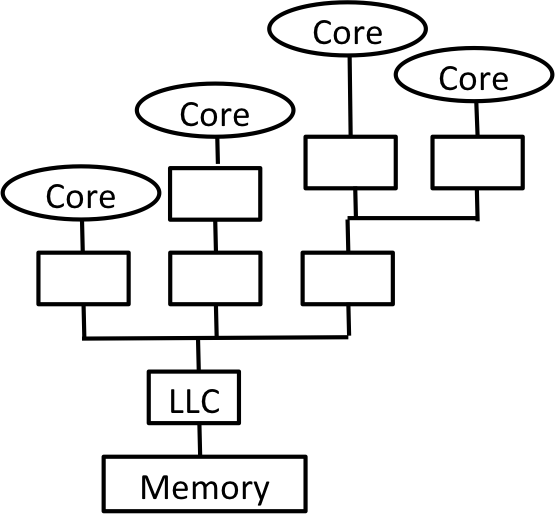
\includegraphics[scale=.4]{hierarchy}
\caption{Logical topology}
\label{hierarchy}
\end{subfigure}
\begin{subfigure}{.45\linewidth}
\centering
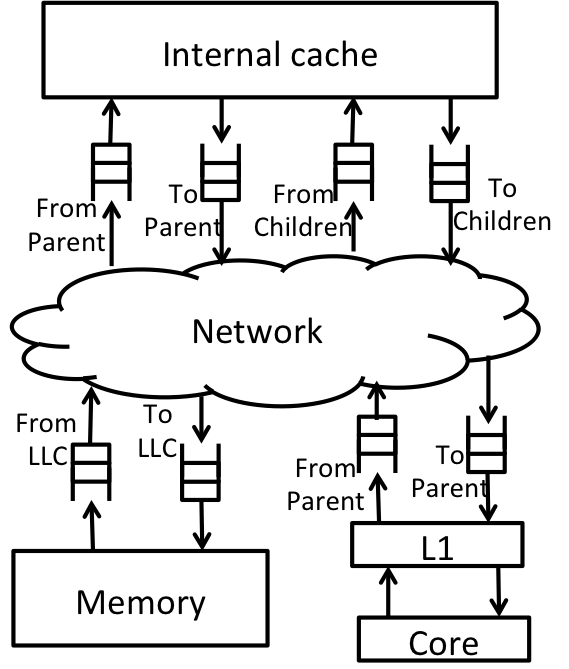
\includegraphics[scale=.4]{physical}
\caption{Physical topology}
\label{physical}
\end{subfigure}
\caption{Logical and physical topology of cache hierarchies}
\end{figure}

In this paper we will consider systems where caches logically form a tree
hierarchy and caches are \emph{inclusive}, that is, if a cache contains address
$a$ then its parent is guaranteed to contain address $a$, though the parent may
have stale data for $a$ (Figure \ref{hierarchy}). Physically the system looks
like a collection of caches connected to a packet switched network (Figure
\ref{physical}). Caches typically contain data and state for each cache line,
and have two pairs of channels for communicating with parent and children
caches. For the lowest level caches (L1's) the channels for communicating with
children are connected to processors, while for the last-level caches the
channels for communicating with the parents are connected to the memory. 

Every cache, unless it is an L1 cache, has a directory which contains
information about the state of its children caches. The cache state-changes to
maintain coherence are orchestrated by passing requests and responses between
the caches using the local directory information.  Unlike bus-based protocols
which lock the bus till all the required state transitions are done thereby
ensuring atomicity of state transitions, in a distributed protocol,
requests and responses are split leading to transient states. This creates
scenarios not present in bus-based protocols, which can lead to coherence
violations or deadlocks, if the protocol is not designed or implemented
carefully.

Several factors contribute to the difficulty of designing protocols for such
distributed, hierarchical and packet-switched systems:

\begin{enumerate}
\item Lots of concurrent events must be dealt with without a central authority
to impose a sequence on events;
\item The state on which transitions are based conceptually is physically
distributed and cannot be accessed atomically;
\item Physical network may block the transmission of a message because of lack
of communication buffers or head-of-the-line blocking;
\item The cache or directory may reach a state in which a particular message
cannot be handled, \ie, an incomplete set of transition rules may cause the protocol
to deadlock.
\end{enumerate}

As examples of problems in designing correct protocols, we describe several
concrete and familiar scenarios from two-level systems (a private L1 cache for
each processor and a shared L2 with a directory). States $M, S$ and $I$ have their
usual meaning in MSI protocol ($M$ represents read and write permissions for an
address, $S$, read-only permissions and $I$, no permission)

\noindent \emph{Example 1:} A cache in state $S$ for a line gets a store
request from the processor and sends an upgrade-to-$M$ request to L2.  L2 may
eventually send an upgrade-to-$M$ response. The response would signify that the
states in the other caches for that line \emph{were} $I$. But the messages take
time to propagate and the response is necessarily based on the old states of
other caches -- the current state of another cache may be $M$, which means two
cores can write to the same location simultaneously, violating cache coherence.

\noindent \emph{Example 2:} A cache in state $S$ for a line gets a store
request from the processor and sends an upgrade-to-$M$ request to L2. Instead
of getting an upgrade-to-$M$ response, the cache may receive a request from L2
asking this cache to go to $I$ state (invalidate request)-- this could have
happened if the directory in L2 is serving some other cache's request to go to
$M$ state for the same line. It is not easy to determine the correct behavior
of the former cache on receiving the invalidate request -- whether it should
ignore the invalidate request and wait for a response to its request or whether
it should invalidate the line. Would ignoring the invalidate request lead to a
deadlock?

\noindent \emph{Example 3:} A cache receives an invalidate request from the
L2 for a line that is not present in the cache. Is such a request even
possible? The directory does not have access to the up-to-date state of the
cache, and so can potentially make this request. How should a cache handle this
request; should it drop such a request, or respond saying that it does not have
the line?

These examples give a glimpse of the complexity of designing and implementing a
correct cache coherence protocol in a distributed setting.  Even for a 2-level
cache hierarchy, designing and implementing the protocol is non-trivial; the
problem gets greatly exacerbated in large multi-level cache system. 

In this paper, we present a substantially easier method to design cache
coherence protocols for such systems. The user specifies a protocol for a cache
hierarchy as sequential methods to process requests. It is not distributed, so the protocol procedure can simultaneously or \emph{atomically}
examine and change the state of all the caches in the system. We then
systematically transform such a protocol description into a distributed protocol. The resulting protocol is presented as a collection
of cooperating sequential methods which operate on ``cache objects''.  These
sequential methods communicate with each other via blocking \emph{send} and
\emph{receive} commands and thus can get suspended. Our transformation is based
on preserving some invariants which guarantee that each request eventually gets
a response and thus, our threads can never wait indefinitely.  It has been
shown using the Coq theorem prover \cite{}, that the distributed protocol we
derive is correct.  Both the transformation procedure and the proof are
parameterized by the number of cache levels and the number of caches in each
level of the hierarchy as well as by a predicate which involves a local
``compatibility of state'' test. A discussion of the formal proof is beyond the
scope of this paper. 

It should be noted that the generality of our procedure comes from the fact
that we do not assign any meaning to a coherence state beyond upgrades and
downgrades. Thus, how or why a particular cache state implies that a particular
address may not be present in any other cache stems from protocol specific
``compatibility of state'' check. 

The main contributions of this paper are: 1. An automatic procedure to refine a
centralized MSI protocol into protocols for
distributed, hierarchical, cache system with packet-switching; 2. Specification
of the requirements that ensure the correctness of the generated protocol;
3. A discussion of the invariants that simplifies the proof of correctness of
the protocol considerably;
4. Giving a provable lower bound on the number of network virtual channels and
buffers to avoid deadlocks; and 5. Showing that our procedure does not
introduce any overhead over direct implementation of these protocols. We think
that our method of designing protocols substantially reduces the required
effort in implementing provably correct protocols. 

\paragraph{Paper organization:} Section \ref{sec:GlobalMsi} describes the MSI
protocol for a hierarchy of caches using nonsuspensive sequential methods. We
use it a specification for proving the correctness of distributed MSI
protocols. Section \ref{sec:DistributedMsi} systematically transforms the
protocol in Section \ref{sec:GlobalMsi} into a distributed protocol. Section
\ref{sec:network} specifies the network, resource and other requirements that
are needed for the distributed MSI protocol. We also give the minimum virtual
channel requirements to ensure the requirements specified in Section
\ref{sec:network}. We show that these formally verified family of protocols
require no extra state bits, nor extra message transfers compared to other
published implementations.  Section \ref{sec:properties} gives a set of
desirable global properties or invariants that are needed to easily establish
the correctness of the distributed protocol.
%It also lists core properties of the distributed protocol that are needed to establish the invariants.
In Section \ref{sec:related}, we present some of the related work and finally
in Section \ref{sec:conclusion}, we present some directions for future work.
